\documentclass[a4paper,12pt,twoside]{book}
\usepackage{graphicx}
\usepackage{fancyhdr}
\usepackage[font = scriptsize, bf]{caption}
\usepackage[english]{babel}
\usepackage[utf8x]{inputenc}
\usepackage[parfill]{parskip}
\usepackage{amsmath, amssymb}
\usepackage{moreverb}
\usepackage{algorithm} %
\usepackage{algpseudocode}
\usepackage[usenames,dvipsnames]{color}
\usepackage[swapnames]{frontespizio}
\usepackage{url}
\usepackage{setspace}
\usepackage{eqparbox,array}
\usepackage{siunitx}
\usepackage{subfigure} 
\usepackage{wrapfig}
\usepackage{amsthm}
\usepackage{eurosym}
\usepackage{hyperref} 

\renewcommand{\algorithmiccomment}[1]{  //\emph{\textcolor{Gray}{#1}}}


% Sistema i margini per lasciare più spazio di rilegatura
\addtolength{\oddsidemargin}{+1,3cm} 
\addtolength{\evensidemargin}{-1,3cm} 
\onehalfspacing

% Imposta lo stile della prima pagina del capitolo
\fancypagestyle{plain} {
    \fancyhead{}
    \fancyfoot[LE,RO]{\thepage}
    \renewcommand{\headrulewidth}{0pt}
}

\DeclareMathOperator*{\argmax}{arg\,max}
\newcommand{\compInterfacciaDB}{Data Interface}
\newcommand{\compLoader}{Loader}
\newcommand{\compMatrix}{Matrix Creator}
\newcommand{\compTermsSel}{Terms Selector}
\newcommand{\compPosition}{Position Calculator}
\newcommand{\compClustering}{Clustering Component}
\newcommand{\compEvolution}{Evolution Discoverer}

% \newtheorem{thm}[equation]{Theorem}
\newtheorem{thm}{Theorem}[chapter]
\newtheorem{exmp}{Example}[chapter]
\newtheorem{defn}{Definition}[chapter]
\newtheorem{prp}{Property}[chapter]



\hyphenation{ti-me-win-dow}

\graphicspath{{./Immagini/}}


\begin{document}

% frontespizio
\begin{frontespizio}
  \Istituzione{University of Bari ``Aldo Moro''}
  \Logo[3.5cm]{Immagini/logo_uni.jpeg}
  \Divisione{Department of Computer Science}
  \Scuola{Master's Degree in Computer Science}
  \Titolo{Argument Mining}
  \Sottotitolo{Artificial Intelligence}
  \NCandidato{Student}
  \Candidato{Christopher Piemonte}
  \NRelatore{Professor}{Professors}
  \Relatore{Stefano Ferilli}
  \Piede{Academic year 2019-2020}
\end{frontespizio}

% \IfFileExists{Tesi-frn.pdf}{}{%
% 	\immediate\write18{pdflatex Tesi-frn}
% }

\IfFileExists{\jobname-frn.pdf}{}{%
\immediate\write18{pdflatex \jobname-frn}}

\pagestyle{fancy}
\fancyfoot{}
\fancyfoot[LE,RO]{\thepage}
\fancyhead{}
\renewcommand{\headrulewidth}{0pt}
\headheight = 15pt
\frontmatter

% indice
\tableofcontents
\afterpage{\null\newpage}


\frontmatter	
\mainmatter

% Imposta lo stile di intestazione e piè di pagina dei capitoli
\fancyfoot{}
\fancyhead{}
\fancyhead[LE,RO]{\slshape \leftmark}
\fancyfoot[LE,RO]{\thepage}
\renewcommand{\headrulewidth}{1pt}
\renewcommand{\chaptermark}[1]{%
\markboth{\thechapter.\ #1}{}}


% !TEX encoding = UTF-8
% !TEX TS-program = pdflatex
% !TEX root = ../Tesi.tex
% !TEX spellcheck = it-IT

%*******************************************************
% Introduzione
%*******************************************************
\cleardoublepage
\chapter*{Introduzione}
L'argomentazione rappresenta un approccio al ragionamento nei casi in cui si dispone di conoscenza inconsistente, e può essere considerata come un metodo per gestire l’incertezza. Infatti, l’idea alla base dell'argomentazione è quella di valutare il motivo per cui un fatto sia considerato vero analizzando gli argomenti e le relazioni che intercorrono tra essi per valutarne la certezza. Tale processo può essere visto come una forma di ragionamento riguardo gli argomenti per determinarne i più accettabili. Sebbene il termine argomentare possa intuitivamente richiamare diversi significati come quello del ragionamento a partire da premesse fino alle conclusioni o l'esprimere la propria opinione in una discussione, un argomento non si lega a particolari strutture ma in senso astratto è qualsiasi cosa che può attaccare o essere attaccata da un altro argomento. Per tale motivo, un Argumentation Framework può essere adeguato a rappresentare diverse situazioni. La possibilità dell'Argumentation Framework di poter rappresentare diverse situazioni ha portato, nel tempo, alla proposta di estensioni che ponessero attenzione su diversi aspetti, come i tipi di relazione che possono sussistere o la quantificazione della forza di una relazione tra due argomenti.

La capacità di argomentare costituisce una caratteristica fondamentale nel discorso umano. Sia discutendo con altre persone che scrivendo un commento sui Social Media, gli argomenti sono onnipresenti, nella vita reale tanto quanto nel World Wide Web. L'Argumentation Theory è un ramo dell'Intelligenza Artificiale finalizzato a fornire un modello formale per la rappresentazione, la costruzione e la semantica delle argomentazioni. Nella sua forma più semplice, l’Argumentation Framework (AF) di Dung, consiste nel determinare insiemi coerenti di argomenti all'interno di un grafo, composto da entità astratte (gli argomenti) e relazioni binarie di attacco tra queste, fornendo un insieme di semantiche per verificare particolari proprietà ad esso relative \cite{dung1995acceptability}. 

Problema fondamentale risulta quindi la costruzione automatica di argomenti dalle fonti dati disponibili, che possono essere più o meno strutturate. La quantità crescente di dati sul web implica che l'analisi manuale di questi contenuti, inclusi dibattiti e argomenti, è diventata ormai irrealizzabile. L'Argument Mining affronta questo problema sviluppando soluzioni che automatizzano, o almeno facilitano, il processo di costruzione di Argument Framework da testo libero. Per costruire AF ci interessano generalmente due problemi:

\begin{itemize}
    \item l'identificazione degli argomenti
    \item l'identificazione delle relazioni tra gli argomenti.
\end{itemize}

L'Argument Mining è un compito complesso in quanto il linguaggio naturale non presenta una struttura facilmente individuabile.

% da aggiungere parti relative a impl e lavoro

\chapter{Argumentation Theory}
\label{cap:capitolo1}
% !TEX encoding = UTF-8
% !TEX TS-program = pdflatex
% !TEX root = ../Tesi.tex

%************************************************

%************************************************


\section{Argumentation}



\chapter{Mining dai Social Media}
\label{cap:capitolo2}
% !TEX encoding = UTF-8
% !TEX TS-program = pdflatex
% !TEX root = ../Tesi.tex

%************************************************

%************************************************
Segue un overview del metodo generale utilizzato, in sezione \ref{section:approcci} e degli approcci specifici, in sezione \ref{section:data_sources}, per ogni Social Media in esame da cui è stato estratto un argumentation framework.

\section{Metodologie di Mining}
\label{section:approcci}
L'estrazione di argomenti prende in esame la struttura che i commenti in uno specifico Social Network possono assumere. In tutte le fonti analizzate un commento può considerarsi una risposta ad un solo altro commento, questo restituisce una struttura ad albero che, partendo dal nodo radice, si dirama attraverso relazioni di risposta. Di seguito viene descritta l'estrazione dell'albero dei commenti in sezione \ref{subsection:albero_commenti} ed un tentativo di estrazione di un grafo considerando come nodi gli utenti in sezione \ref{subsection:grafo_utenti}.

\subsection{Albero dei commenti}
\label{subsection:albero_commenti}
Per la costruzione dell'albero dei commenti serve costruire un grafo orientato della conversazione $\mathcal{G = ⟨V, E⟩}$, dove i nodi $v \in \mathcal{V}$ sono commenti ed esiste un arco $(v_1,v_2) \in \mathcal{E}$ se il commento $v_1$ risponde al commento $v_2$.

La struttura dell'albero può variare in base alla sorgente dei dati in esame, ad esempio alcuni Social Network pongono un limite al numero di livelli dell'albero, principalmente per motivi di presentazione.
Estrarre delle semantiche da Argumentation Framework ricavati dall'albero della conversazione equivale ad estrarre i commenti che soddisfano i requisiti delle varie semantiche.

\subsection{Grafo degli utenti}
\label{subsection:grafo_utenti}
Invece di considerare i commenti come argomenti, può essere considerato argomento ogni utente nella conversazione, e creare archi nel Argumentation Framework risultante tra due utenti se un utente ha risposto almeno una volta ad un altro utente. Più formalmente costruire un grafo orientato $\mathcal{G = ⟨V, E⟩}$, dove i nodi $v \in \mathcal{V}$ sono utenti ed esiste un arco $(v_1,v_2) \in \mathcal{E}$ se l'utente $v_1$ ha risposto almeno una volta all'utente $v_2$.

In questo modo se ogni commento nell'albero della conversazione ha un utente univoco, l'Argumentation Framework risultante sarà comunque un albero, mentre se un utente risponde ad almeno due (o più) utenti il suo nodo nell'$AF$ avrà due (o più) archi uscenti, e se più commenti dello stesso utente vengono risposti da due (o più) utenti, il suo nodo nell'$AF$ avrà due (o più) archi entranti.
Estrarre delle semantiche da Argumentation Framework ricavati dal grafo degli utenti equivale ad estrarre gli utenti che soddisfano i requisiti delle varie semantiche.

\subsection{Pesi delle relazioni}
\label{subsection:weight}
Le relazioni di risposta nell'albero dei commenti vengono pesate in base alla combinazione di similarità e sentiment dei commenti della relazione.

\subsubsection{Similarity}
La \textit{similarity} è ricavata attraverso l'embedding dei testi dei commenti ricavati da un modello di Word2Vec pre-addestrato sulle news di Google \cite{googlenewsmodel}. Gli Word Embedding sono un insieme di tecniche per la rappresentazione vettoriale delle parole di un vocabolario, introdotti per la prima volta in \cite{mikolov2013distributed}, i quali sono capaci di catturare il contesto delle parole all'interno di un documento attraverso la \textit{distributional semantics}. I vettori risultanti codificano proprietà linguistiche nello spazio vettoriale e nella distanza tra di essi, ad esempio è possibile fare analogie come mostrato in figura \ref{fig:analogy}.

\begin{figure}
    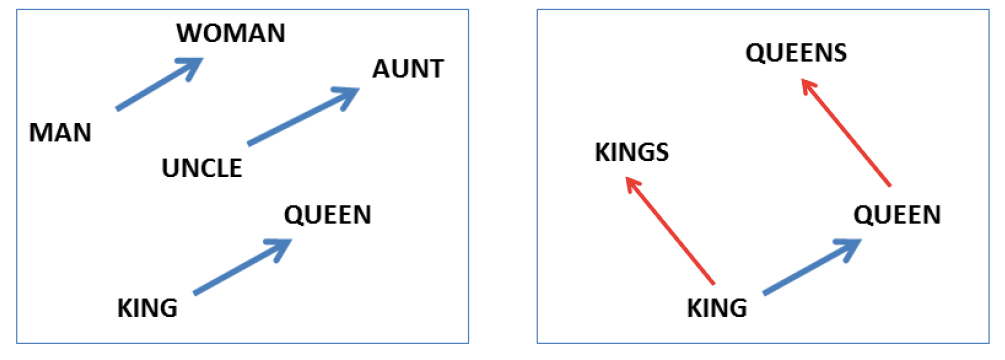
\includegraphics[width=\linewidth]{Immagini/king-queen.png}
    \caption{Analogie tra vettori.}
    \label{fig:analogy}
\end{figure}

L'emebedding dei testi dei commenti è ottenuto facendo la media degli embedding delle parole contenute. Infine la similarità tra due testi $c_1$ e $c_2$ si ricava con:

$$cosineSimilarity(c_1, c_2) = \frac{c_1 \cdot c_2}{||c_1|| ||c_2||}$$

che restituirà quindi un risultato compreso $\in [0, 1]$.

\subsubsection{Sentiment}
La \textit{sentiment analysis} si riferisce all'utilizzo dell'elaborazione del linguaggio naturale per identificare, estrarre e quantificare sistematicamente informazioni soggettive. L'analisi del sentiment è ampiamente applicata per analizzare social media per una varietà di applicazioni. Il valore è ricavato attraverso VADER \cite{hutto2014vader} uno strumento di analisi del sentimento basato su regole che è ideato specificamente per individuare la polarità nei testi espressi nei social media, ad esempio:

    $$sentiment(\ "\textbf{:)}" \ ) = 0.4588$$
    $$sentiment(\ "\textbf{:(}" \ ) = -0.4404$$

che restituirà quindi un risultato compreso $\in [-1, 1]$.

\subsubsection{Peso finale}
Il peso finale dell'arco è ottenuto prendendo in considerazione la similarità tra i commenti, in modo da pesare di più commenti che parlano dello stesso argomento e di meno commenti che parlano di argomenti diversi, ed il sentiment in modo da capire se i commenti sono in accordo o in disaccordo attraverso:

$$weight = similarity_{c_1 c_2} \cdot sentiment_{c_1} \cdot sentiment_{c_2}$$

che restituirà quindi un risultato compreso $\in [-1, 1]$.

\section{Analisi dei Social Media}
\label{section:data_sources}

\subsection {Twitter} %%%%%%%%%%%%%%%%%%%%%%%%%%%%%%%%%%%%%%%%%%%

Lo scraping del sito Web è vietata dal Twitter Terms of Service, quindi l'unico modo rimane l'accesso tramite API. Per accedere alla piattaforma delle API di twitter è necessario creare un Twitter developer account ed in seguito creare dal portale una applicazione nella quale si dichiara lo scopo dello dell'accesso ai contenuti e si richiedono i relativi permessi. Una volta ottenuta l'approvazione, vengono rilasciati delle credenziali per l'autenticazione agli endpoint, ovvero:

\begin{itemize}
    \item consumer key
    \item consumer secret
    \item access token
    \item access token secret
\end{itemize}

I contenuti messi a disposizione sono i Tweet pubblici, cercando parole chiave specifiche attraverso le Search API o chiedendo esempi di Tweet a determinati account attraverso le User API. Inoltre è possibile richiedere tweet specifici conoscendone l'id.

\subsubsection{Overview}
Al momento non è disponibile l'accesso alle conversazioni, la richiesta di tweet tramite le Search API o le User API restituisce solo un sottoinsieme dei tweet ed inoltre c'è un limite al numero di richieste giornaliere. Questo rende difficile cercare di ricostruire le conversazioni dai tweet restituiti dalla query. 

\subsubsection{Ricostruire la conversazione}
\label{ricostruire-conv}
La richiesta ad un determinato topic restituisce un campione di massimo 1000 tweet recenti.
Fra gli attributi presenti nei tweet è presente il campo \textbf{"in reply to status id"} che, se presente, contiene l'id del tweet al quale il tweet corrente sta rispondendo. Questo id può essere utilizzato per cercare di ricostruire la conversazione, facendo una richiesta tramite API per avere il tweet risposto e, se questo a sua volta risponde ad un altro tweet, continuare a seguire la catena di risposte (la conversazione). Per qualsiasi tweet con questo campo, possiamo:
\begin{itemize}
    \item trovare il tweet a cui quello corrente sta rispondendo, quindi ripetere la procedura per ogni tweet con questo attributo avvalorato in modo da ottenere delle sequenze di tweet.
    \item Una volta create le sequenze di tweet, se queste contengono elementi in comune, unire le sequenze creando un grafo della conversazione.
    \item Valutare la bontà della conversazione ottenuta mediante euristiche come il numero di elementi (tweet) nel grafo, la presenza di diramazioni o il numero di utenti distinti.
\end{itemize}

Quindi costruire grafo orientato della conversazione $\mathcal{G = ⟨V, E⟩}$, dove i nodi $v \in \mathcal{V}$ sono tweet ed esiste un arco $(v_1,v_2) \in \mathcal{E}$ se l'attributo \textbf{"in reply to status id"} di $v_1$ contiene l'id di $v_2$.

Tuttavia le API forniscono l'accesso solo ad un campione dei tweet, quindi potrebbe non essere possibile recuperare dei tweet quando si tenta di ricostruire la conversazione. Un'altra limitazione proviene dal numero di tweet iniziale che è possibile ottenere in risposta alla query, che risulta essere massimo 1000, dei quali è necessario filtrare i tweet che contengono il campo \textbf{"in reply to status id"} avvalorato, numero che può variare di molto (di solito circa il 10\%). Inoltre le conversazioni risultano quasi sempre essere sequenze lineari di nodi, ovvero grafi con archi in entrata $\leq 1$ ed archi in uscita $\leq 1$ come rappresentato in figura \ref{fig:comment-twitter} ed il grafo ricostruito cambia in base al momento della richiesta.

\begin{figure}[ht]
    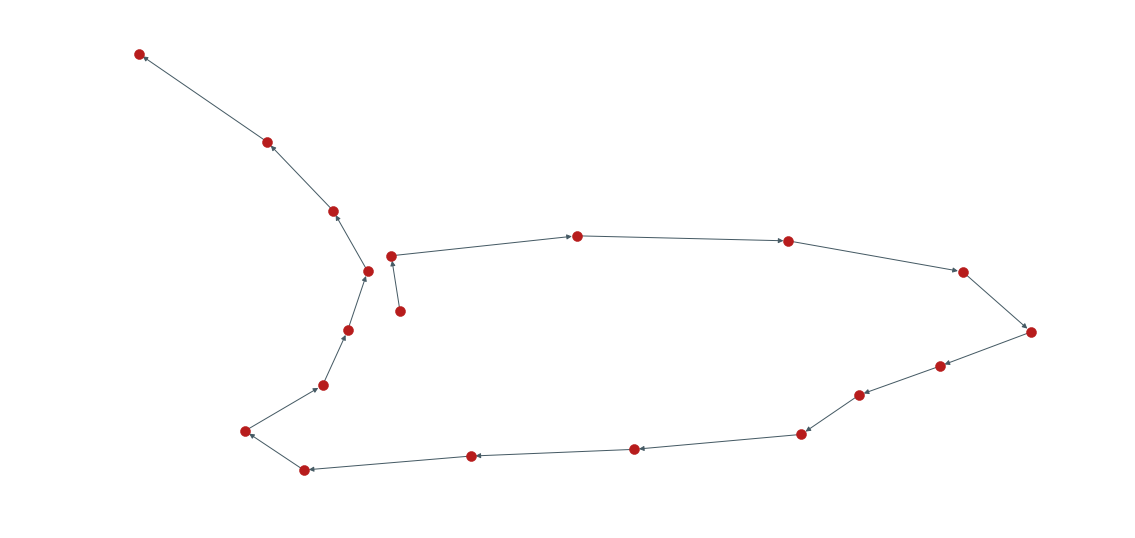
\includegraphics[width=\linewidth]{Immagini/twitter.png}
    \caption{Rappresentazione del grafo della conversazione, utilizzando come nodi i commenti.}
    \label{fig:comment-twitter}
\end{figure}

\subsubsection {Utenti come nodi}
Un altro approccio utilizzato, indipendente dalle funzionalità messe a disposizione da Twitter o dalle Twitter API, consiste nel considerare gli utenti in una conversazione come nodi e creare un arco orientato tra due utenti se esiste almeno un tweet di risposta tra i due, più formalmente: costruire un grafo orientato $\mathcal{G = ⟨V, E⟩}$, dove i nodi $v \in \mathcal{V}$ sono utenti ed esiste un arco $(v_1,v_2) \in \mathcal{E}$ se esiste almeno un tweet con utente $v_1$ e con l'attributo \textbf{"in reply to status id"} contenente l'id di un tweet appartenente all'utente $v_2$.

Anche qui si ripropongono i problemi presentati nella sezione precedente \ref{ricostruire-conv}, tuttavia il grafo risultante presenta nodi con archi in entrata $\geq 1$ ed archi in uscita $\geq 1$, come rappresentato in figura \ref{fig:users-twitter}.

\begin{figure}[ht]
    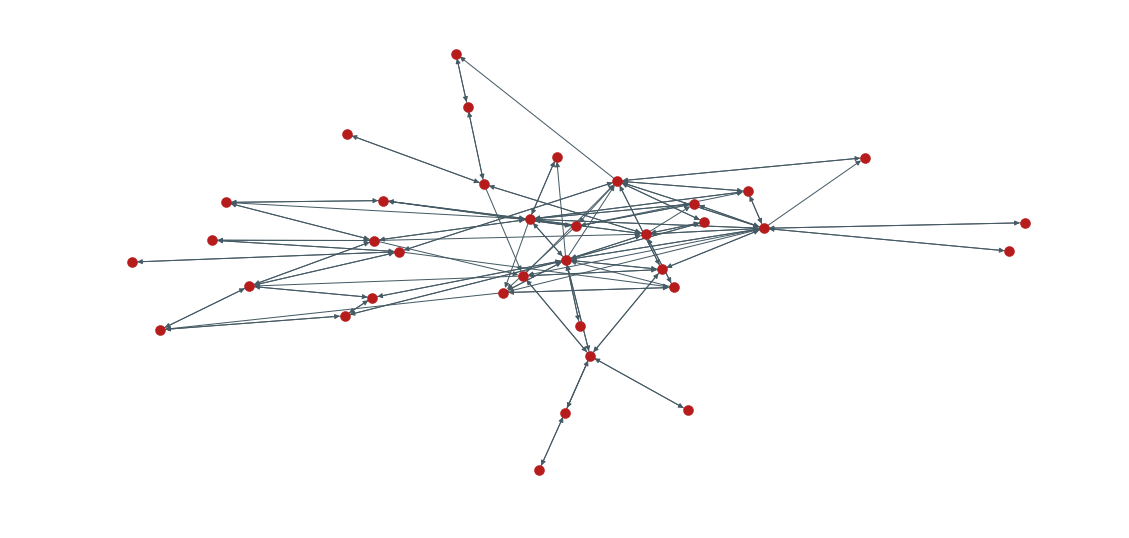
\includegraphics[width=\linewidth]{Immagini/twitter-users.png}
    \caption{Rappresentazione del grafo della conversazione, utilizzando come nodi gli utenti.}
    \label{fig:users-twitter}
\end{figure}



%%%%%%%%%%%%%%%%%%%%%%%%%%%%%%%%%%%%%%%%%%%%%%%%%%%%%%%%%%%%%%%
%%%%%%%%%%%%%%%%%%%%%%%%%%%%%%%%%%%%%%%%%%%%%%%%%%%%%%%%%%%%%%%
%%%%%%%%%%%%%%%%%%%%%%%%%%%%%%%%%%%%%%%%%%%%%%%%%%%%%%%%%%%%%%%
%%%%%%%%%%%%%%%%%%%%%%%%%%%%%%%%%%%%%%%%%%%%%%%%%%%%%%%%%%%%%%%
%%%%%%%%%%%%%%%%%%%%%%%%%%%%%%%%%%%%%%%%%%%%%%%%%%%%%%%%%%%%%%%


\subsection {Stackoverflow} %%%%%%%%%%%%%%%%%%%%%%%%%%%%%%%%%%%%%%%%%%%

\begin{itemize}
    \item create account at https://stackapps.com/
    \item register an app
    \item b
\end{itemize}

\subsubsection {Overview}
\subsubsection {API}

\subsubsection {Commenti}
\subsubsection {Utenti}


%%%%%%%%%%%%%%%%%%%%%%%%%%%%%%%%%%%%%%%%%%%%%%%%%%%%%%%%%%%%%%%
%%%%%%%%%%%%%%%%%%%%%%%%%%%%%%%%%%%%%%%%%%%%%%%%%%%%%%%%%%%%%%%
%%%%%%%%%%%%%%%%%%%%%%%%%%%%%%%%%%%%%%%%%%%%%%%%%%%%%%%%%%%%%%%
%%%%%%%%%%%%%%%%%%%%%%%%%%%%%%%%%%%%%%%%%%%%%%%%%%%%%%%%%%%%%%%
%%%%%%%%%%%%%%%%%%%%%%%%%%%%%%%%%%%%%%%%%%%%%%%%%%%%%%%%%%%%%%%

\subsection {Reddit} %%%%%%%%%%%%%%%%%%%%%%%%%%%%%%%%%%%%%%%%%%%

\begin{itemize}
    \item create account at 
    \item register an app
    \item b
\end{itemize}


\subsubsection {Overview}
\subsubsection {API}

\subsubsection {Commenti}
\subsubsection {Utenti}

% Fatti generati argument/1, attac- k/2, support/2, rel_weight/3

% descrizione vader e altri componenti utilizzati



\chapter{Ranking extensions}
\label{cap:capitolo3}
% !TEX encoding = UTF-8
% !TEX TS-program = pdflatex
% !TEX root = ../Tesi.tex
% !TEX spellcheck = it-IT

%************************************************

%************************************************

% ranking extensions


\section {Generazione estensioni}
La generazione delle estensioni all'interno di un grafo di argomenti equivale all'estrarre sottoinsiemi di nodi coerenti fra di loro secondo i vincoli imposta dalla semantica. Il mining dei social media permette di mappare in questo dominio i commenti o gli utenti, estraendo quindi sottoinsiemi di questi che soddisfano i requisiti. 

Dipendentemente dal tipo di conversazione estratta i gruppi di commenti/utenti coerenti fra di loro possono avere diverse interpretazioni. All'interno di un dibattito politico potrebbero rappresentare l'accordo o il disaccordo con un certo argomento portato dal politico, in un post su di una serie tv potrebbe rappresentare il gradimento verso un particolare personaggio o sottotrama. 

\subsection {Implementazione}
Per l'implementazione delle estensioni è stato utilizzato il framework \textit{Arguer} \cite{}. Il sistema implementato in Prolog permette di importare Argumentation Framework sotto forma di basi di conoscenza prolog e calcolare le semantiche. 

È stato scelto di utilizzare il sistema Arguer in quanto era già presente come framework per il calcolo delle semantiche e l'implementazione di un tale sistema da zero avrebbe richiesto lo l'impegno tale da costituire un progetto a se stante.

%%%%%%%%%%%%%%%%%%%%%%%%%%%%%%%%%%%%%%%%%%%%%%%%%%%%%%%%%%%%%%%
%%%%%%%%%%%%%%%%%%%%%%%%%%%%%%%%%%%%%%%%%%%%%%%%%%%%%%%%%%%%%%%
%%%%%%%%%%%%%%%%%%%%%%%%%%%%%%%%%%%%%%%%%%%%%%%%%%%%%%%%%%%%%%%
%%%%%%%%%%%%%%%%%%%%%%%%%%%%%%%%%%%%%%%%%%%%%%%%%%%%%%%%%%%%%%%
%%%%%%%%%%%%%%%%%%%%%%%%%%%%%%%%%%%%%%%%%%%%%%%%%%%%%%%%%%%%%%%

\section {Ranking delle estensioni}
La generazione delle semantiche si limita a verificare i requisiti imposti dalla semantica ed a restituire un insieme di insiemi di nodi. Tutti i sottoinsiemi che soddisfano i vincoli sono egualmente importante. Collocando l'interpretazione degli argomenti in un dato dominio e guidati da una determinata applicazione, potrebbe essere utile dare una priorità a certe estensioni in base a delle metriche dei suoi nodi ad esempio o alla lunghezza del sottoinsieme. 

Le metriche possono prendere in considerazione diversi aspetti dell argumentation framework, dalla topologia del grafo al testo del commento. Fra le graph based quelle implementate sono:

\begin{itemize}
    \item \textbf{Distanza fra i nodi del sottoinsieme}: calcolata come la distanza fra tutte le possibili coppie all'interno della estensione (divisa per la lunghezza della estensione).

    \item \textbf{indegree nel grafo di difesa}: un nodo $\mathcal{V}$ è difeso da un altro nodo $\mathcal{U}$ se esiste un altro nodo $\mathcal{W}$ tale che $\mathcal{W}$ attacca $\mathcal{V}$ e $\mathcal{U}$ attacca $\mathcal{W}$. Mentre per BAF e BWAF oltre la relazione di difesa è considerata anche la relazione di supporto.

    \item \textbf{closeness nel grafo di difesa}: valore attribuito ad un nodo calcolando la media di tutti gli shortest path con sorgente quel nodo e destinazione gli altri nodi.

    \item \textbf{indegree nel grafo di attacchi}: per questa metrica vengono considerati solo le relazione di attacco, andando a considerare migliori i nodi con indegree basso.

    \item \textbf{closeness nel grafo di attacchi}: stesso valore descritto sopra ma calcolato nel grafo considerando solo le relazioni di attacco.
\end{itemize}


Il valore aggiunto di una metrica è da attribuire a logiche di business in base alla specifica interpretazione e conoscenza che si ha degli argomenti.



\chapter{Sviluppi futuri}
\label{cap:capitolo4}
% !TEX encoding = UTF-8
% !TEX TS-program = pdflatex
% !TEX root = ../Tesi.tex
% !TEX spellcheck = it-IT

%************************************************

%************************************************

% sviluppi futuri
L'implementazione del sistema di Argumentation Mining e del sistema prolog per il ranking delle estensioni è stata soggetta a molte scelte dovute allo stato dell'arte del periodo di sviluppo e ad uno stampo generale che si è voluto dare alle due parti del progetto. Con l'evoluzione delle tecniche e tramite applicazione del sistema ad un caso reale è possibile prendere scelte più ponderate ed adatte al contesto. Così come ampliare la scelta di metriche e fonti dati da cui attingere per la creazione del grafo di argomenti.


\section{Mining}
\label{section:ranking}

\subsection {Fonti} 
I social media rappresentano una fonte importante per l'Argumentation Mining, l'aggiunta di altre fonti potrebbe essere guidato da caratteristiche specifiche offerte dalle specifiche piattaforme. I social media presentano una grande opportunità però per motivi di visualizzazione spesso impongono dei vincolo nella struttura dei commenti. Potrebbe essere utile esplorare l'estrazione di argomenti da altre fonti web o in genere testuali. Un'idea potrebbe essere trovare un fonte dati con delle caratteristiche per le quali la creazione del grafo emerga ed abbia valore all'interno di un contesto di analisi, nei testi di un decreto o di una causa legale.

\subsection {Generazioni pesi delle relazioni} 
I pesi delle relazioni sono in funzione del sentiment e della similarità dei testi dei due commenti della relazione. In questo caso è stato utilizzato vader \cite{hutto2014vader} come sentiment analyzer perchè trainato sui social network, ma questo potrebbe cambiare in base alla fonte dati.

La similarità invece è calcolata tramite la creazione di word embedding delle parole attraverso l'algoritmo word2vec \cite{} ed in seguito attraverso la creazione di embedding per l'intero testo attraverso la media degli embedding delle parole. Questo porta a considerare simili testi che contengono parole simili attraverso la Distributional Semantic ovvero utilizzate in contesti simili.

L'introduzione di nuovi algoritmi allo stato dell'arte per il language modeling potrebbe portare miglioramenti nel comprensione del significato della frase e di conseguenza in una più accurata generazione di relazioni e pesi. In particolar modo ELMo \cite{elmo} e BERT \cite{bert} possono essere addestrati ed utilizzati per estrarre rappresentazioni vettoriali delle frasi.




%%%%%%%%%%%%%%%%%%%%%%%%%%%%%%%%%%%%%%%%%%%%%%%%%%%%%%%%%%%%%%%
%%%%%%%%%%%%%%%%%%%%%%%%%%%%%%%%%%%%%%%%%%%%%%%%%%%%%%%%%%%%%%%
%%%%%%%%%%%%%%%%%%%%%%%%%%%%%%%%%%%%%%%%%%%%%%%%%%%%%%%%%%%%%%%
%%%%%%%%%%%%%%%%%%%%%%%%%%%%%%%%%%%%%%%%%%%%%%%%%%%%%%%%%%%%%%%
%%%%%%%%%%%%%%%%%%%%%%%%%%%%%%%%%%%%%%%%%%%%%%%%%%%%%%%%%%%%%%%

\section {Ranking}

\subsection {Nuove funzioni di ranking}

Sempre nell'ambito della elaborazione dei testi, ELMo \cite{elmo} e BERT \cite{bert} possono essere utilizzati per produrre nuove metriche prendendo in considerazione i testi dei commenti all'interno della stessa estensione, dando valore maggiore alle estensioni con argomenti con testi simili tra di loro.

La topologia del grafo può essere utilizzata attraverso la scoperta di cluster con algoritmi di Clustering / community detection ed in seguito utilizzarli come ground truth per calcolare metriche come la homogeneity, completeness fra i cluster e le estensioni. 

Ci sono molte metriche provenienti dalla graph theory che possono essere implementate, così come il calcolo del page rank potrebbe essere utile in alcuni contesti applicativi.

L'effettiva utilità di queste funzioni di scoring rimane comunque da valutare in base al caso in esame. Alcune potrebbero essere puramente teoriche senza avere un riscontro effettivo nel preferire un estensione rispetto ad un altra.



% \chapter{Critical analysis}
% \input{Capitoli/Conclusioni}


\bibliographystyle{plain}
\bibliography{Bibliografia}

\end{document}
